%%%%%%%%%%%%%%%%%%%%%%%%%%%%%%%%%%%%%%%%%%%%%%%%%%%%%%%%%%%%%%%%%%%%%%
%%                     module
%%%%%%%%%%%%%%%%%%%%%%%%%%%%%%%%%%%%%%%%%%%%%%%%%%%%%%%%%%%%%%%%%%%%%%
\subsection{\glyph{Submap}}\label{sec:submap}

\corr{A \glyph{submap} is used to encapsulate processes (including all types of nodes and edges) within one glyph.
The \glyph{submap} hides its content to the users, and displays only \corr{input terminals (or ports)}{\glyph{submap terminals} (\sect{submapTerminal})}, linked to \glyph{EPNs} (\sect{EPNs}) \add{or \glyph{compartments} (\sect{compartment})}.
A \glyph{submap} is not equivalent to an \glyph{omitted process} (\sect{omitted}).
\luna{032819 maybe later can we have another section called implementation notes? for this kind of information?}
In the case of an SBGN map that is made available through a software tool, the content of a \glyph{submap} may be available to the tool.
A user could then ask the tool to expand the \glyph{submap}, for instance by clicking on the icon representing the \glyph{submap}.
The tool might then expand and show the \glyph{submap} within the same map (on the same canvas), or it might open it in a different canvas. In the case of an SBGN description made available in a book or a website, the content of the submap may be available on another page, possibly accessible via an hyperlink on the \glyph{submap}.
}{
A \glyph{submap} is used to encapsulate a map (including all types of nodes and edges) within one glyph.
As such, it is not equivalent to an \glyph{omitted process} (\sect{omitted}).
The \glyph{submap} hides the content of this map to the users, and displays only \glyph{submap terminals} (\sect{submapTerminal}).
% , linked to \glyph{EPNs} (\sect{EPNs}) or \glyph{compartments} (\sect{compartment}) of the map using \glyph{equivalence arcs} (\sect{equivalenceArc}).
In the case of an SBGN description that is made available through a software tool, the map enclosed by the  \glyph{submap} may be available to the tool.
A user could then ask the tool to expand this map in a different canvas, for instance by clicking on the \glyph{submap}.
In the case of an SBGN description made available in a book or a website, the content of the map may be available on another page, possibly accessible via an hyperlink on the \glyph{submap}.
}
\rougny{If we make a distinction between the tag glyph and the submap terminal glyph, it is difficult to allow for submap expansion inside of the submap glyph (because submap terminals would also become tags, and that would become complicated).
Since there are also no examples in V1.3 where a submap is expanded inside a submap glyph, maybe it is best to just forbid that.
I rewrote the paragraph and this entire section as if it was forbidden.
Maybe it should be discussed.
UD: This doesn't sound like expanding is forbidden to me. Also, I am not sure if it's a good idea to talk about software/tool issues. I agree that this stuff should be designed to address tool issues but I am not sure if this new version is the right time.

VT: When expanding a submap glyph to show it's content in the main map, wouldn't the submap terminals and tags disappear? That is how I understood this. So it is up to the tool, I would think, to take care of this 'mapping' and 'reasoning'. SBGN provides a way to connect both maps through the terminal and tag, no?
}

\begin{glyphDescription}

\glyphSboTerm
SBO:0000395 ! encapsulating process

\add{
\glyphIncoming
None.
}

\add{
\glyphOutgoing
None.
}

\glyphContainer
\corr{
The \glyph{submap} is represented as a square box, to remind that it is fundamentaly a process.
}{
A \glyph{submap} is represented by a rectangular shape, to remind that it is fundamentally a process.
}

\glyphLabel
\corr{
The identification of the \glyph{submap} is carried by an unbordered box containing a string of characters.
The characters may be distributed on several lines to improve readability, although this is not mandatory.  The label box has to be attached to the center of the container box.
}{
A \glyph{submap} is identified by a label that is an unbordered box containing a string of characters.
The characters may be distributed on several lines to improve readability.
The centre of the label must be placed on the centre of the shape.
The label may extend outside of the shape.
}

\glyphAux
\corr{A \glyph{submap} carries labeled terminals. When the submap is represented folded, those terminals are linked to external EPNs (section~\ref{sec:EPNs}) or containers (section~\ref{sec:CNs}). In the unfolded view, exposing the internal structure of the submap, a set of \glyph{tags} point to the corresponding internal EPNs (section~\ref{sec:EPNs}) or containers (section~\ref{sec:CNs}).
}{
A \glyph{submap} must carry one or more \glyph{submap terminals} (\sect{submapTerminal}), each linked to an \glyph{EPN} (\sect{EPNs}) or \glyph{compartment} (\sect{compartment}) of the map using an \glyph{equivalence arc} (\sect{equivalenceArc}).
}
\end{glyphDescription}

\begin{figure}
\begin{center}
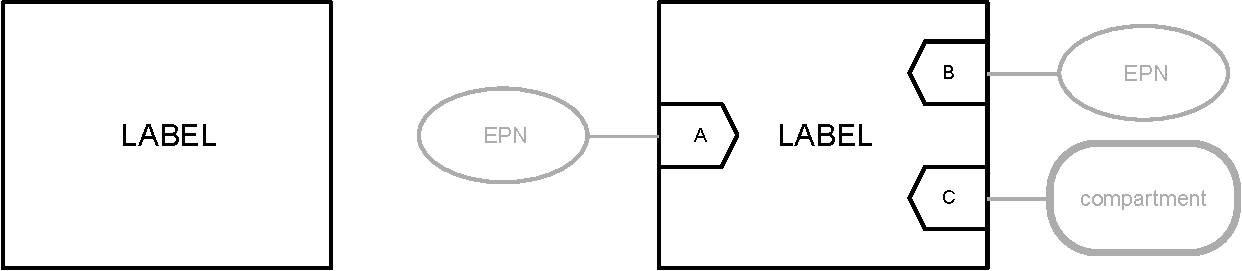
\includegraphics[scale=0.7]{images/submap.pdf}
\caption{The \PD glyph for \glyph{submap}, shown plain and unadorned on the left, and with three \glyph{submap terminals} on the right.}
\label{fig:submap}
\end{center}
\end{figure}

\corr{The following map represents a \glyph{submap} that transforms glucose into fructose-6-phosphate. The \glyph{submap} carry five terminals, four linked to EPNs and one linked to a \glyph{compartment}. The latter is particularly important in the case of EPNs present only in a \glyph{compartment} enclosed in a \glyph{submap}, and that are not linked to terminals themselves. Note that the terminals do not define a ``direction'', such as input or output. The flux of the reactions is determined by the context.
}{
\fig{folded} represents a \glyph{submap} that encapsulates processes transforming glucose into fructose-6-phosphate.
The \glyph{submap} carries five \glyph{submap terminals}, four linked to \glyph{EPNs} and one linked to a \glyph{compartment}.
The latter is particularly important in the case of \glyph{EPNs} present only in a \glyph{compartment} enclosed in a \glyph{submap}, and that are not linked to \glyph{submap terminals} themselves.
Note that the \glyph{submap terminals} do not allow defining a ``direction'' for the flux of the processes enclosed in the \glyph{submap}, which is solely determined by the context as in \fig{folded}.
}

\begin{figure}
\begin{center}
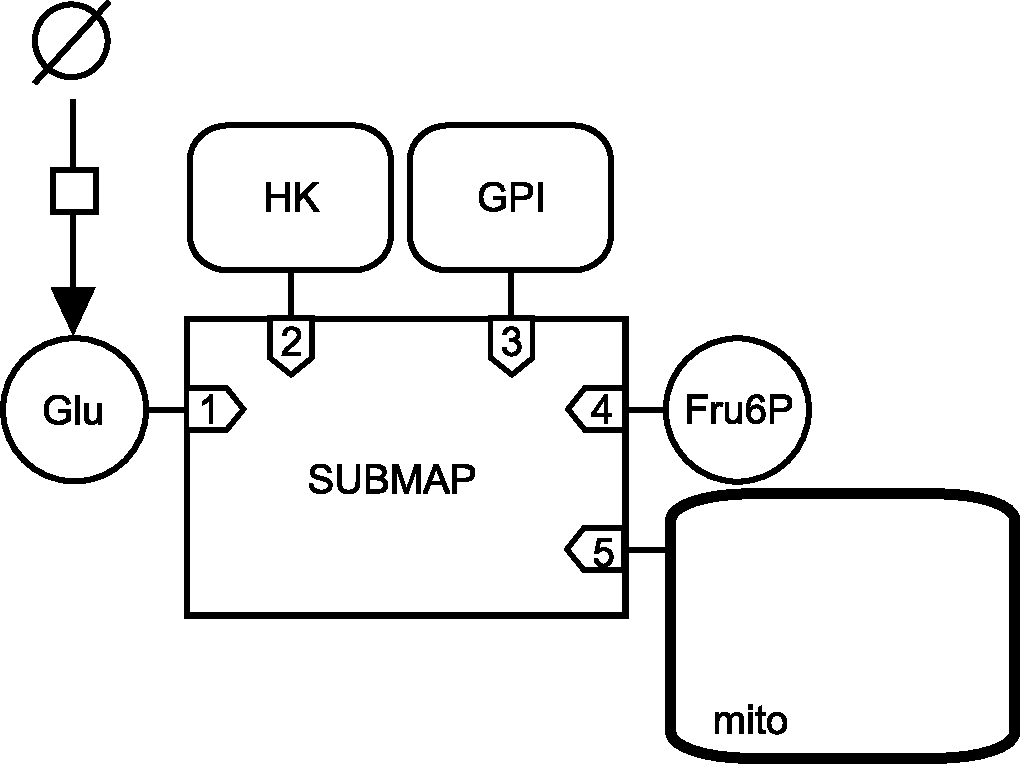
\includegraphics[scale=0.8]{examples/submap-folded.pdf}
\caption{\corr{Example of a \glyph{submap} with contents elided}{Example of a \glyph{submap} encapsulating processes that transform glucose into fructose-6-phosphate.
The map enclosed by the \glyph{submap} is shown in \fig{unfolded}, whose \glyph{tags} are referred to by the \glyph{submap terminals} decorating the present \glyph{submap} glyph.
\dogrusoz{... decorating the main (or present) map (not submap).
AR: here submap refers to the glyph. Added glyph at the end to make that clear.}
}}
\label{fig:folded}
\end{center}
\end{figure}

\corr{The following map represents the unfolded version of the above, displaying the reactions enclosed in the module \emph{in the same canvas}. Note the terminal 5, linking the compartment ``mitom'' of the submap to the to the compartment ``mito'' outside the submap. The compartment containing Glu6P is implicitly defined as the same than the compartment containing Glum and Fru6pm. There is no ambiguity because if Glu and Fru6m were in different compartments, one of them should have been defined within the submap.
}{
The map in \fig{unfolded} represents the map enclosed in the \glyph{submap} of \fig{folded}.
Note that the tag 5 links the mitochondria \glyph{compartment} in this map to the mitochondria \glyph{compartment} of the main map in \fig{unfolded}.
% \dogrusoz{... the tag 5 links (or associates) the mitochondria ...}
The \glyph{compartment} containing glucose-6-phosphate is implicitly defined as the same as the \glyph{compartment} containing glucose and fructose-6-phosphate.
There is no ambiguity because if glucose and fructose-6-phosphate were in different \glyph{compartments}, at least one of them would have been linked to a \glyph{submap terminal} of the \glyph{submap} of \fig{folded}.
% \dogrusoz{... different compartments, at least one of them would have been linked to a submap terminal of the submap.}
}

\begin{figure}
\begin{center}
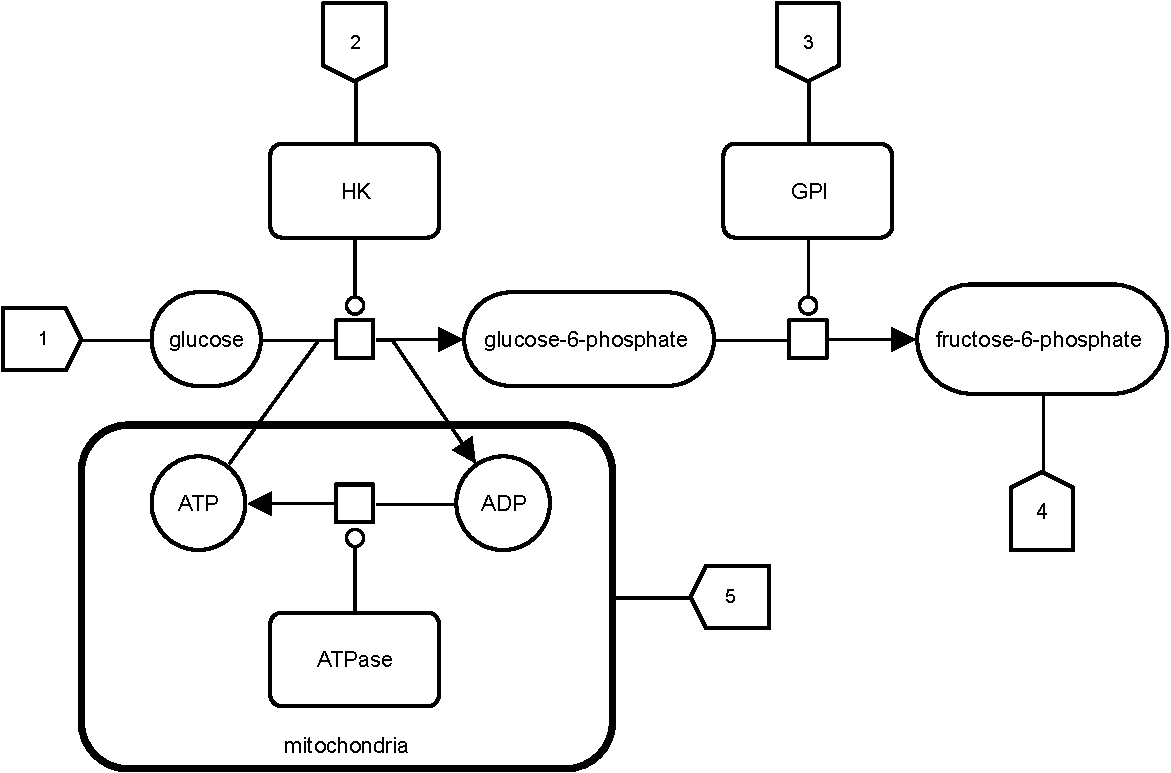
\includegraphics[scale=0.8]{examples/submap-unfolded.pdf}
\caption{\corr{Example of an unfolded submap. The unfolded submap corresponds to the folded submap of \fig{folded}.}{Example of a map with \glyph{tags}, showing that it is enclosed in a \glyph{submap} of another map (here, the one of \fig{folded}).}}
\label{fig:unfolded}
\end{center}
\end{figure}

% The following map represents another unfolded version of the above, displaying the reactions enclosed in the submap \emph{in a different canvas}. Here, the anything outside the submap has disappeared, and the internal \glyph{tags} are not linked to the corresponding external \glyph{units of information}.
%
% \begin{center}
% \scalebox{0.5}{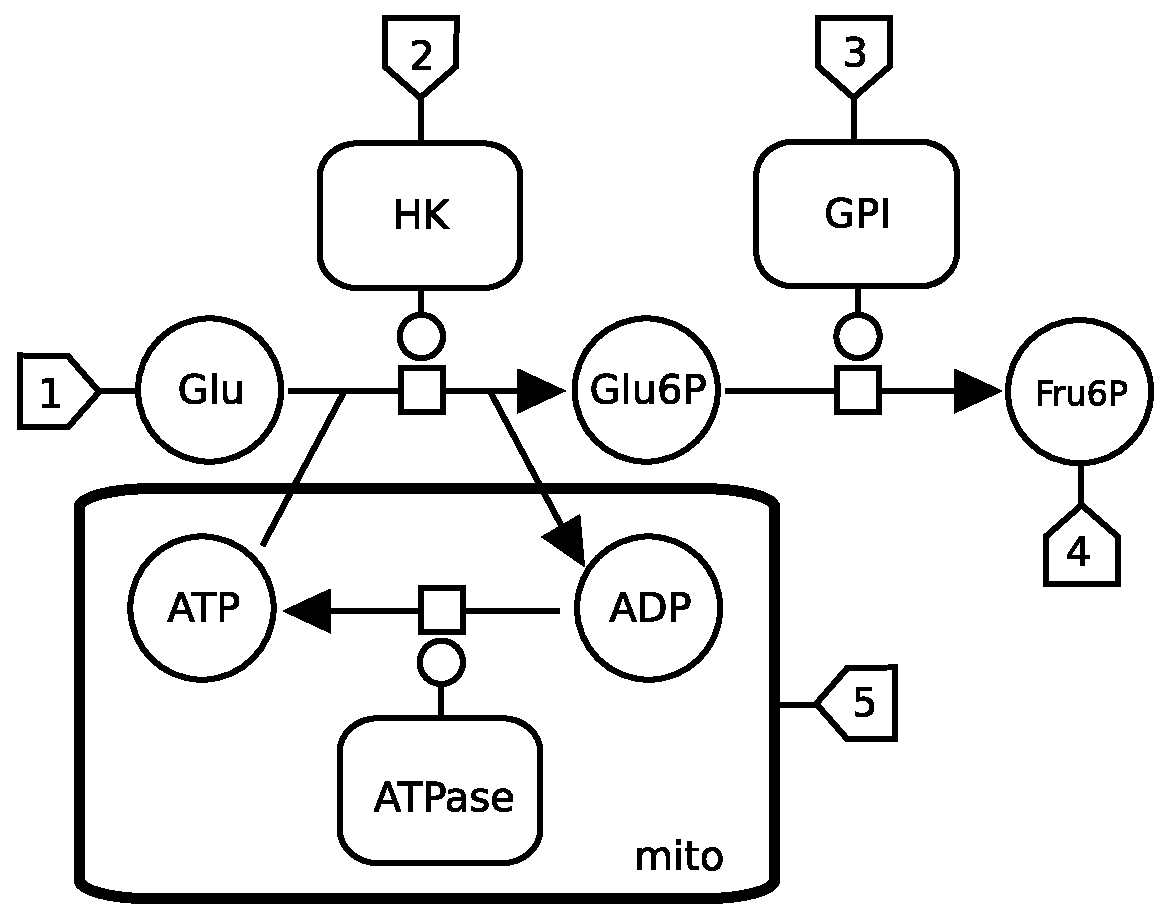
\includegraphics{examples/submap-dissociated.eps}}
% \end{center}
% \normalcolor

